% Compilation : pdflatex Changement_de_referentiel.tex (deux fois).
% Document autonome : texte, formules et figures TikZ modifiables.
% Les reperes Source renvoient aux pages du manuscrit.
\documentclass[11pt,a4paper]{article}
\usepackage[utf8]{inputenc}
\usepackage[T1]{fontenc}
\usepackage[provide=*,french]{babel}
\usepackage[scaled=.95]{helvet}
\renewcommand{\familydefault}{\sfdefault}
\usepackage{amsmath,amssymb,esint,array,tabularx}
\usepackage{geometry}
\geometry{left=15mm,right=15mm,top=18mm,bottom=18mm,headheight=14pt,headsep=6mm}
\usepackage{fancyhdr,lastpage,tikz}
\usetikzlibrary{arrows.meta,calc,decorations.pathreplacing,decorations.pathmorphing,decorations.markings,patterns}
\usepackage[most]{tcolorbox}
\usepackage{enumitem,titlesec,needspace,hyperref}
\hypersetup{hidelinks,pdftitle={Changement de référentiel},pdfsubject={Cours de physique}}
\pagestyle{fancy}\fancyhf{}
\fancyhead[L]{\small Physique M2 - Changement de référentiel - inspiré par les cours de Mme Mesnil}
\fancyhead[R]{\small\thepage/\pageref{LastPage}}
\fancyfoot[R]{\small PC-PC*}
\renewcommand{\headrulewidth}{0pt}
\setlength{\parindent}{0pt}\setlength{\parskip}{5pt}
\setlength{\abovedisplayskip}{7pt}\setlength{\belowdisplayskip}{7pt}
\setlist[itemize]{leftmargin=5mm,itemsep=3pt,topsep=3pt,label=\(\rightarrow\)}
\setlist[enumerate]{leftmargin=6mm,itemsep=3pt,topsep=3pt}
\renewcommand{\thesection}{\Roman{section}}
\renewcommand{\thesubsection}{\thesection.\arabic{subsection}}
\titleformat{\section}{\Large\bfseries}{\thesection.}{.4em}{}
\titleformat{\subsection}{\large\bfseries}{\thesubsection.}{.4em}{}[\titlerule]
\titleformat{\subsubsection}{\normalsize\bfseries}{\alph{subsubsection})}{.5em}{}
\titlespacing*{\section}{0pt}{11pt}{6pt}
\titlespacing*{\subsection}{0pt}{9pt}{5pt}
\titlespacing*{\subsubsection}{0pt}{8pt}{4pt}
\newtcolorbox{cadre}[1][]{enhanced,sharp corners,colback=white,colframe=black,boxrule=1.1pt,left=7pt,right=7pt,top=5pt,bottom=5pt,before skip=7pt,after skip=7pt,#1}
\newtcolorbox{exemple}[1][]{enhanced,sharp corners,colback=white,colframe=black,boxrule=.7pt,left=8pt,right=8pt,top=6pt,bottom=6pt,before skip=8pt,after skip=8pt,#1}
\tcbset{etoiles/.style={width=\dimexpr\linewidth-22mm\relax,overlay={\node[anchor=west,inner sep=0pt,font=\small] at ([xshift=2mm]frame.east) {\(#1\)};}}}
\newcommand{\dd}{\mathrm d}
\newcommand{\vv}{\vec v}
\newcommand{\grad}{\overrightarrow{\mathrm{grad}}}
\newcommand{\pd}[2]{\frac{\partial #1}{\partial #2}}
\newcommand{\ux}{\vec u_x}\newcommand{\uy}{\vec u_y}\newcommand{\uz}{\vec u_z}
\newcommand{\cste}{\mathrm{cste}}
\newcommand{\titr}[1]{\par\textbf{\underline{#1}}\par\nopagebreak[3]}
\newcommand{\planpart}[2]{\par\vspace{5pt}{\bfseries #1. #2}\par}
\newcommand{\plansub}[2]{\hspace*{7mm}{\itshape #1) #2}\par}
\newcommand{\plansubsub}[1]{\hspace*{15mm}{\itshape #1}\par}
\tikzset{>=Stealth,every node/.style={font=\small},flow/.style={thick,->},edge/.style={thick}}
\newcommand{\etoiles}[1]{\foreach \i in {1,...,#1}{\mathord{\star}\,}}
\newcommand{\R}{\mathcal R}
\newcommand{\Om}{\vec\Omega_{\R'/\R}}
\newcommand{\Os}{\vec\Omega_{S/\R}}
\newcommand{\D}[2]{\left.\frac{\dd #1}{\dd t}\right|_{#2}}
\newcommand{\DD}[2]{\left.\frac{\dd^2 #1}{\dd t^2}\right|_{#2}}
\newcommand{\V}[1]{\vec v_{#1}}
\newcommand{\A}[1]{\vec a_{#1}}
\newcommand{\rep}[1]{\draw[->] (0,0)--(1.15,0);\draw[->] (0,0)--(0,1.3);\draw[->] (0,0)--(-.65,-.8);\node[below right] at (.2,-.15){$#1$};}
\newcommand{\deuxrep}[1]{\begin{tikzpicture}[scale=.75]
\rep{\R}\node[above left,xshift=-2pt] at (0,0){$O$};
\begin{scope}[shift={(4,.3)}]\ifnum#1=1\begin{scope}[rotate=45]\rep{}\end{scope}\node[right] at (.8,-.25){$\R'$};\else\rep{\R'}\fi\node[left] at (0,0){$O'$};\end{scope}
\draw[thick] (1,-1.5)..controls (1.5,-.7) and (2,-1.6)..(2.9,-.8);
\fill (1.9,-1.18) circle(2pt) node[below]{$M$};
\ifnum#1=2\node[above] at (1.9,-1.18){$P$};\fi
\end{tikzpicture}}
\newcommand{\rotationfig}{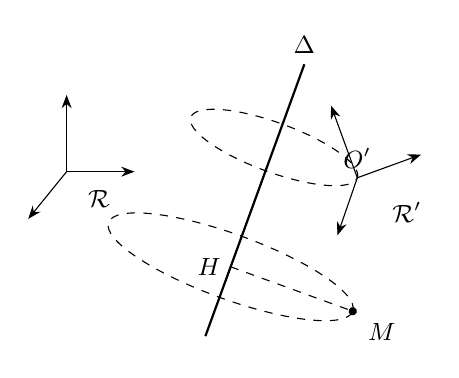
\begin{tikzpicture}[scale=.75]
\begin{scope}[shift={(-3,1)}]\rep{\R}\end{scope}
\begin{scope}[rotate=-20]
\draw[thick] (0,-1.9)--(0,3) node[above]{$\Delta$};
\draw[dashed] (0,1.5) ellipse(1.5 and .42);
\draw[dashed] (0,-.65) ellipse(2.2 and .55);
\coordinate (P) at (2.2,-.65);\coordinate (H) at (0,-.65);
\draw[dashed] (H)--(P);\node[left] at (H){$H$};
\fill (P) circle(2pt) node[below right,xshift=2pt,yshift=-1pt]{$M$};

\begin{scope}[shift={(1.5,1.5)},rotate=40]\rep{}\end{scope}
\node[right] at (2.1,1.1){$\R'$};\node[above] at (1.5,1.5){$O'$};
\end{scope}
\end{tikzpicture}}
\newcommand{\terre}{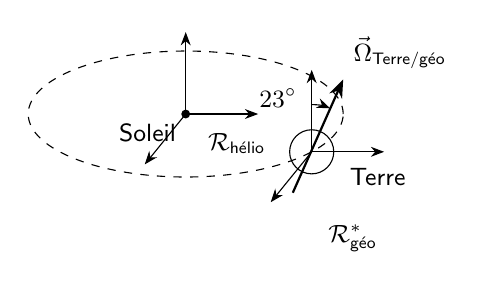
\begin{tikzpicture}[scale=.8]
\draw[dashed] (0,0) ellipse(2.5 and 1);
\rep{\R_{\text{hélio}}}\fill (0,0) circle(2pt) node[below left]{Soleil};
\begin{scope}[shift={(2,-.6)}]
\draw (0,0) circle(.35);
\draw[->] (0,0)--(1.15,0);\draw[->] (0,0)--(0,1.3);\draw[->] (0,0)--(-.65,-.8);
\node[below] at (.65,-1){$\R^*_{\text{géo}}$};
\draw[->,thick] (-.3,-.65)--(.5,1.15) node[above right]{$\vec\Omega_{\text{Terre/géo}}$};
\draw[->] (0,.75) arc(90:67:.75);\node[left] at (-.08,.85){$23^\circ$};
\node[right] at (.45,-.4){Terre};\end{scope}
\end{tikzpicture}}
\begin{document}
{\fontsize{27}{31}\selectfont\bfseries Changement de référentiel en mécanique classique\par}
\vspace{4mm}
\begingroup\setlength{\parskip}{1.4pt}
\par\vspace{5pt}\textbf{Introduction}\par
\planpart{I}{Mouvement d'un solide}
\plansub{1}{Définition d'un solide}
\plansub{2}{Degrés de liberté d'un solide}
\plansub{3}{Mouvement d'un solide}
\plansubsub{a) Solide en translation}
\plansubsub{b) Solide en rotation autour d'un axe fixe}
\plansubsub{c) Cas général}
\planpart{II}{Dérivation d'un vecteur par rapport au temps}
\plansub{1}{Dérivées des vecteurs de base de $\R'$ dans $\R$}
\plansub{2}{Dérivation d'un vecteur quelconque}
\plansub{3}{Composition des vecteurs rotation}
\planpart{III}{Composition des vitesses}
\plansub{1}{Vitesse d'un point dans deux référentiels}
\plansub{2}{Loi de composition des vitesses}
\plansub{3}{Cas d'un référentiel $\R'$ en translation par rapport à $\R$}
\plansub{4}{Cas d'un référentiel $\R'$ en rotation uniforme autour d'un axe fixe dans $\R$}
\planpart{IV}{Composition des accélérations}
\plansub{1}{Accélération d'un point dans deux référentiels}
\plansub{2}{Composition des accélérations}
\plansub{3}{Cas d'un référentiel $\R'$ en translation par rapport à $\R$}
\plansub{4}{Cas d'un référentiel $\R'$ en rotation uniforme autour d'un axe fixe dans $\R$}
\par\vspace{5pt}\textbf{Annexe}\par
\endgroup
% Source : page 1.
\section*{Introduction}
La cinématique étudie le mouvement. Le mouvement est relatif : il dépend du référentiel d'étude.
\begin{exemple}
La chute d'une balle dans un train en est un exemple.
\end{exemple}
\begin{exemple}
\titr{Exemple : une roue de vélo}
\begin{center}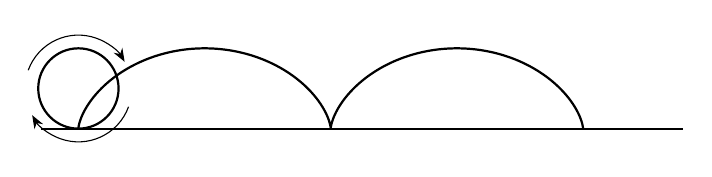
\begin{tikzpicture}[scale=.6]
\draw[thick] (-.8,0)--(12.8,0);
\draw[thick,domain=0:720,samples=161,smooth,variable=\t] plot ({.85*(\t*pi/180-sin(\t))},{.85*(1-cos(\t))});
\draw[thick] (0,.85) circle(.85);\begin{scope}[shift={(0,.85)}]\draw[->] (160:1.13) arc(160:30:1.13);\draw[->] (-20:1.13) arc(-20:-150:1.13);\end{scope}
\end{tikzpicture}\end{center}
La trajectoire est une cycloïde dans $\R$ lié au sol. Elle est circulaire dans le référentiel lié au centre de la roue.
\end{exemple}
L'objectif est de relier les vitesses et les accélérations dans deux référentiels :
\[\V{\R}(M)\longleftrightarrow\V{\R'}(M),\qquad \A{\R}(M)\longleftrightarrow\A{\R'}(M).\]
Un référentiel est l'association d'un repère d'espace (un solide) et d'une horloge. En mécanique classique, on ignore l'horloge.
% Source : pages 2-3.
\section{Mouvement d'un solide}
\subsection{Définition d'un solide}
Un solide indéformable est un solide idéal tel que
\[\forall M\in S,\ \forall N\in S,\qquad MN=\cste\quad\text{au cours du temps}.\]
\subsection{Degrés de liberté d'un solide}
Les degrés de liberté d'un système sont les paramètres nécessaires, suffisants et indépendants pour déterminer sans ambiguïté sa position et son mouvement.
\begin{exemple}
\titr{Exemples}
Un point matériel possède :
\begin{itemize}
\item deux degrés de liberté sur une surface ;
\item un degré de liberté sur un fil ;
\item trois degrés de liberté s'il est libre dans l'espace.
\end{itemize}
Un solide possède six degrés de liberté : trois pour la position de $G$ et trois angles d'Euler (hors programme).
\begin{center}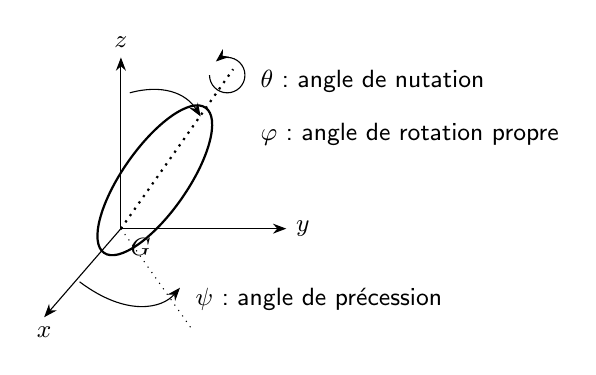
\begin{tikzpicture}[scale=.75]
\draw[->] (0,0)--(-1.3,-1.5) node[below]{$x$};\draw[->] (0,0)--(2.8,0) node[right]{$y$};\draw[->] (0,0)--(0,2.9) node[above]{$z$};
\draw[thick,rotate=-35] (0,1) ellipse(.55 and 1.5);\draw[dotted,thick] (0,0)--(1.9,2.7);\draw[dotted] (0,0)--(1.2,-1.7);\node[below right] at (0,0){$G$};
\draw[->] (.15,2.3)..controls (.7,2.45) and (1.1,2.3)..(1.35,1.9);\node[right,align=left] at (2.2,2.5){$\theta$ : angle de nutation};
\draw[->] (-.7,-.9)..controls (.1,-1.5) and (.7,-1.35)..(1,-1);\node[right] at (1.1,-1.2){$\psi$ : angle de précession};
\draw[->] (1.5,2.6) arc(180:490:.3);\node[right] at (2.2,1.6){$\varphi$ : angle de rotation propre};
\end{tikzpicture}\end{center}
\end{exemple}
\subsection{Mouvement d'un solide}
\subsubsection{Solide en translation}
Un solide $S$ est en translation dans un référentiel $\R$ si
\[\forall M\in S,\ \forall N\in S,\qquad\overrightarrow{MN}=\cste\quad\text{au cours du temps}.\]
\titr{Conséquences}
Soit $O$ un point fixe de $\R$.
\begin{align*}
\D{\overrightarrow{MN}}{\R}=\vec0
&\Longleftrightarrow \D{\overrightarrow{MO}}{\R}+\D{\overrightarrow{ON}}{\R}=\vec0\\
&\Longleftrightarrow-\V{\R}(M)+\V{\R}(N)=\vec0\\
&\Longleftrightarrow\V{\R}(M)=\V{\R}(N),\qquad\forall M,N\in S.
\end{align*}
Il n'y a que trois degrés de liberté : le mouvement d'un point donne le mouvement du solide.
\titr{Cas particuliers}
\begin{itemize}
\item En translation rectiligne, la vitesse instantanée garde toujours la même direction.
\item En translation rectiligne uniforme, elle conserve la même direction, le même sens et la même norme.
\item En translation circulaire, chacun des points a une trajectoire circulaire.
\end{itemize}
% Source : page 4.
\titr{Hors programme : référentiel barycentrique}
Le référentiel barycentrique $\R^*$, associé à un système $\Sigma$ par rapport à un autre référentiel $\R$, vérifie :
\begin{itemize}
\item $\R^*$ est en translation par rapport à $\R$ ;
\item le centre d'inertie $G$ de $\Sigma$ est fixe dans $\R^*$.
\end{itemize}
\begin{exemple}
\titr{Exemple : une roue, $\Sigma=\text{roue}$}
\begin{center}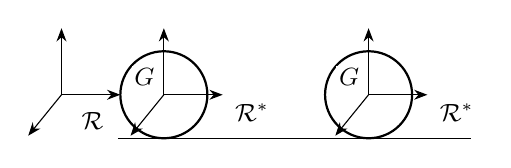
\begin{tikzpicture}[scale=.65]
\begin{scope}[shift={(-2,0)}]\rep{\R}\end{scope}\draw (-.9,-.85)--(6,-.85);
\foreach \x in {0,4}{\begin{scope}[shift={(\x,0)}]\draw[thick] (0,0) circle(.85);\rep{}\node[above left,fill=white,inner sep=1pt] at (-.12,.12){$G$};\node[right] at (1.2,-.35){$\R^*$};\end{scope}}
\end{tikzpicture}\end{center}
\end{exemple}
\begin{exemple}
\titr{Exemple : un ballon de rugby}
\begin{center}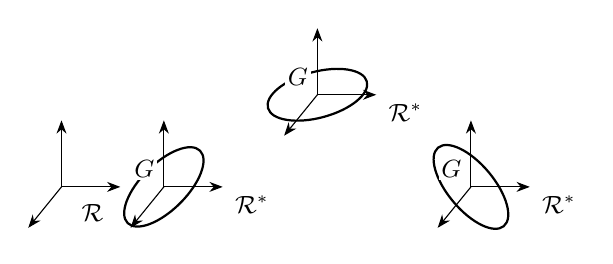
\begin{tikzpicture}[scale=.65]
\begin{scope}[shift={(-2,0)}]\rep{\R}\end{scope}
\foreach \x/\y/\a in {0/0/45,3/1.8/15,6/0/-50}{\begin{scope}[shift={(\x,\y)}]\draw[thick,rotate=\a] (0,0) ellipse(1 and .45);\rep{}\node[above left,fill=white,inner sep=1pt] at (-.12,.12){$G$};\node[right] at (1.2,-.35){$\R^*$};\end{scope}}
\end{tikzpicture}\end{center}
\end{exemple}
\subsubsection{Solide en rotation autour d'un axe fixe}
\begin{center}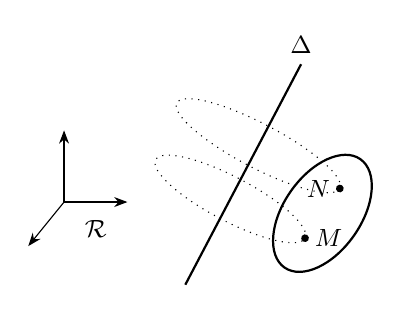
\begin{tikzpicture}[scale=.7]
\begin{scope}[shift={(-3,0)}]\rep{\R}\end{scope}
\draw[thick] (-.8,-1.5)--(1.3,2.5) node[above]{$\Delta$};
\draw[dotted,rotate around={-27.699:(0.0169,0.0559)}] (0.0169,0.0559) ellipse(1.5307 and .4);
\draw[dotted,rotate around={-27.699:(0.5240,1.0220)}] (0.5240,1.0220) ellipse(1.6705 and .4);
\draw[thick,rotate=-35] (1.5,.8) ellipse(.7 and 1.2);
\begin{scope}[rotate=-35]\fill (1.5,.25) circle(2pt) node[right]{$M$};\fill (1.5,1.35) circle(2pt) node[left]{$N$};\end{scope}
\end{tikzpicture}\end{center}
Tous les points $M$ du solide ont une trajectoire circulaire autour de l'axe $\Delta$, avec la même vitesse angulaire $\omega(t)=\dot\theta(t)$.
Il n'y a qu'un seul degré de liberté : l'angle $\theta$. Le sens de $\theta$ est donné par $\vec u_\Delta$.
\begin{center}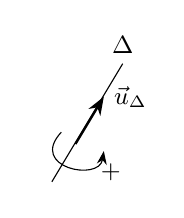
\begin{tikzpicture}[scale=.6]
\draw (-.5,-.8)--(1,1.7) node[above]{$\Delta$};\draw[flow] (0,0)--(.6,1) node[right]{$\vec u_\Delta$};\draw[->] (-.3,.25)..controls (-1,-.5) and (.5,-.8)..(.6,-.15);\node at (.75,-.6){$+$};
\end{tikzpicture}\end{center}
\begin{cadre}\[\Os=\frac{\dd\theta}{\dd t}\vec u_\Delta.\]\end{cadre}
Ce vecteur rotation a une direction constante ; son sens et sa norme peuvent changer.
\titr{Calcul de $\V{\R}(M)$}
La vitesse est différente pour les différents points. $H$ est le projeté orthogonal de $M$ sur $\Delta$. On utilise la base cylindrique associée à $\Delta$ : $(M,\vec u_r,\vec u_\theta,\vec u_\Delta)$.
\begin{center}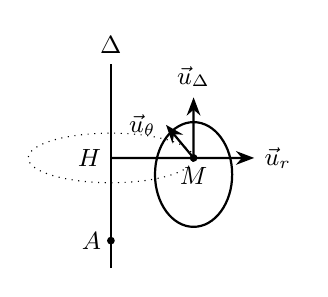
\begin{tikzpicture}[scale=.7]
\draw[thick] (0,-1.5)--(0,2.2) node[above]{$\Delta$};\draw[dotted] (0,.5) ellipse(1.5 and .45);
\coordinate (M) at (1.5,.5);\draw[thick] (0,.5)--(M);\node[left] at (0,.5){$H$};\fill (0,-1) circle(2pt) node[left]{$A$};\fill (M) circle(2pt) node[below]{$M$};
\draw[flow] (M)--(2.6,.5) node[right]{$\vec u_r$};\draw[flow] (M)--(1.5,1.6) node[above]{$\vec u_\Delta$};\draw[flow] (M)--(1,1.1) node[left]{$\vec u_\theta$};
\draw[thick] (1.5,.2) ellipse(.7 and .95);
\end{tikzpicture}\end{center}
\[\V{\R}(M)=HM\,\dot\theta\,\vec u_\theta.\]
Si $M\in\Delta$, alors $\V{\R}(M)=\vec0$.
\[\V{\R}(M)=\Os\wedge\overrightarrow{HM}.\]
\begin{cadre}\[\V{\R}(M)=\Os\wedge\overrightarrow{AM}.\]\end{cadre}
Ici, $A\in\Delta$ est fixe dans $\R$.
% Source : page 6.
\begin{align*}
\D{\overrightarrow{MN}}{\R}
&=\D{\overrightarrow{MO}}{\R}+\D{\overrightarrow{ON}}{\R}\\
&=-\V{\R}(M)+\V{\R}(N)\\
&=-\Os\wedge\overrightarrow{AM}+\Os\wedge\overrightarrow{AN}\\
&=\Os\wedge\bigl(\overrightarrow{AN}-\overrightarrow{AM}\bigr).
\end{align*}
\begin{cadre}\[\D{\overrightarrow{MN}}{\R}=\Os\wedge\overrightarrow{MN},\qquad\forall M,N\in S.\]\end{cadre}
\begin{exemple}[breakable]
\titr{Remarque hors programme : particule chargée dans un champ $\vec B$ uniforme}
\[m\frac{\dd\vec v}{\dd t}=q\vec v\wedge\vec B.\]
Le travail est nul, donc $E_c=\cste$ et $v=\cste$. On considère un mouvement plan, avec $\vec v_0\perp\vec B$ à $t=0$.
\titr{Base de Frenet}
\[\frac{\dd\vec v}{\dd t}=\underbrace{\frac{\dd v}{\dd t}\vec T}_{=\vec0}+\frac{v^2}{R}\vec N.\]
\[\frac{mv^2}{R}\vec N=q\vec v\wedge\vec B=qv\vec T\wedge B\vec u_z.\]
On suppose la charge $q$ positive.\par
On obtient $R=\dfrac{mv}{qB}$ : la trajectoire est circulaire.
\titr{Autre méthode}
\[\frac{\dd\vec v}{\dd t}=\underbrace{-\frac qm\vec B}_{=\Os}\wedge\vec v.\]
On retrouve la pulsation cyclotron : le vecteur vitesse tourne autour d'un axe.
\end{exemple}
% Source : pages 7-8.
\subsubsection{Cas général}
On peut toujours définir un vecteur rotation instantané $\Os(t)$, dont le sens, la direction et la norme dépendent du temps.
\nopagebreak[4] La relation suivante est admise dans le cas général :\nopagebreak[4]
\begin{cadre}\[\D{\overrightarrow{MN}}{\R}=\Os(t)\wedge\overrightarrow{MN},\qquad\forall M,N.\]\end{cadre}
Le cas général n'est pas explicitement au programme. Sont au programme :
\begin{itemize}
\item la translation de $S$ dans $\R$ :
\[\Os=\vec0\quad\Longrightarrow\quad\D{\overrightarrow{MN}}{\R}=\vec0;\]
\item la rotation de $S$ autour d'un axe fixe : $\Os$ a une direction constante.
\end{itemize}
Le mouvement d'un solide est en général très compliqué. On décompose le problème en deux :
\begin{enumerate}
\item le mouvement de $G$ dans $\R$ ;
\item le mouvement de $S$ dans $\R^*$ : $G$ est fixe et l'axe instantané de rotation passe par $G$.
\end{enumerate}
\begin{exemple}
\titr{Exemple}
\begin{center}\terre\end{center}
$G$ est le centre d'inertie de la Terre. La Terre tourne autour de l'axe polaire.
\end{exemple}
\section{Dérivation d'un vecteur par rapport au temps}
\begin{center}\begin{tikzpicture}[scale=.7]
\draw[->] (0,0)--(1.4,0) node[right]{$x$};\draw[->] (0,0)--(0,1.3) node[above]{$y$};\draw[->] (0,0)--(-.7,-.9) node[below]{$z$};\node at (.7,-.5){$\R$};
\begin{scope}[shift={(5,0)},rotate=-35]\draw[->] (0,0)--(1.4,0) node[right]{$x'$};\draw[->] (0,0)--(0,1.3) node[above]{$y'$};\draw[->] (0,0)--(-.7,-.9) node[below]{$z'$};\end{scope}\node at (5,-1){$\R'$};
\end{tikzpicture}\end{center}
Soit $\vec v$ un vecteur quelconque :
\[\vec v(t)=x(t)\vec x+y(t)\vec y+z(t)\vec z
=x'(t)\vec x'+y'(t)\vec y'+z'(t)\vec z'.\]
\[\D{\vec v}{\R}=\dot x(t)\vec x+\dot y(t)\vec y+\dot z(t)\vec z.\]
\begin{align*}
\D{\vec v}{\R}
&=\dot x'(t)\vec x'+x'(t)\D{\vec x'}{\R}\\
&\quad+\dot y'(t)\vec y'+y'(t)\D{\vec y'}{\R}
+\dot z'(t)\vec z'+z'(t)\D{\vec z'}{\R}.
\end{align*}
\[\D{\vec v}{\R'}=\dot x'(t)\vec x'+\dot y'(t)\vec y'+\dot z'(t)\vec z'.\]
% Source : pages 9-10.
\subsection{Dérivées des vecteurs de base de $\R'$ dans $\R$}
\titr{Cas où $\R'$ est en translation par rapport à $\R$}
\[\D{\vec x'}{\R}=\vec0,\qquad\D{\vec y'}{\R}=\vec0,\qquad\D{\vec z'}{\R}=\vec0.\]
\titr{Cas où $\R'$ est en rotation autour d'un axe $\Delta$ fixe dans $\R$}
\[\D{\vec x'}{\R}=\Om\wedge\vec x',\qquad
\D{\vec y'}{\R}=\Om\wedge\vec y',\qquad
\D{\vec z'}{\R}=\Om\wedge\vec z'.\]
\titr{Cas général (hors programme)}
\[\begin{aligned}
\D{\vec x'}{\R}&=\Om(t)\wedge\vec x',\\
\D{\vec y'}{\R}&=\Om(t)\wedge\vec y',\\
\D{\vec z'}{\R}&=\Om(t)\wedge\vec z'.
\end{aligned}\]
Les expressions sont les mêmes que pour la rotation, mais $\Om$ est variable.
\subsection{Dérivation d'un vecteur quelconque}
\begin{align*}
\D{\vec v}{\R}
&=\dot x'(t)\vec x'+\dot y'(t)\vec y'+\dot z'(t)\vec z'\\
&\quad+x'(t)\D{\vec x'}{\R}+y'(t)\D{\vec y'}{\R}+z'(t)\D{\vec z'}{\R}\\
&=\D{\vec v}{\R'}+x'(t)\Om\wedge\vec x'
+y'(t)\Om\wedge\vec y'+z'(t)\Om\wedge\vec z'.
\end{align*}
\begin{cadre}[etoiles={\etoiles{2}}]
\[\D{\vec v}{\R}=\D{\vec v}{\R'}+\Om\wedge\vec v(t).\]
\end{cadre}
\textbf{Remarque :} si $\R'$ est en translation par rapport à $\R$, alors $\Om=\vec0$ et
\[\D{\vec v}{\R}=\D{\vec v}{\R'}.\]
\textbf{Remarque :} $\D{\vec v}{\R}$ et $\D{\vec v}{\R'}$ sont deux vecteurs différents.
% Source : pages 11-13.
\subsection{Composition des vecteurs rotation}
\begin{center}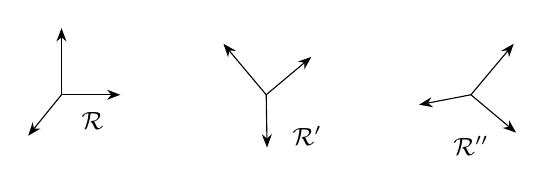
\begin{tikzpicture}[scale=.65]
\rep{\R}\begin{scope}[shift={(4,0)},rotate=40]\rep{}\end{scope}\node at (4.8,-.8){$\R'$};\begin{scope}[shift={(8,0)},rotate=-40]\rep{}\end{scope}\node at (8,-1){$\R''$};
\end{tikzpicture}\end{center}
On veut montrer que :
\begin{cadre}[etoiles={\etoiles{3}}]
\[\vec\Omega_{\R''/\R}=\vec\Omega_{\R''/\R'}+\Om.\]
\end{cadre}
Soit $\vec v(t)$ quelconque.
\begin{align*}
\D{\vec v}{\R}
&=\D{\vec v}{\R''}+\vec\Omega_{\R''/\R}\wedge\vec v\\
&=\underbrace{\D{\vec v}{\R'}}_{=\D{\vec v}{\R''}+\vec\Omega_{\R''/\R'}\wedge\vec v}+\Om\wedge\vec v.
\end{align*}
D'où
\[\D{\vec v}{\R''}+\vec\Omega_{\R''/\R}\wedge\vec v
=\D{\vec v}{\R''}+\vec\Omega_{\R''/\R'}\wedge\vec v+\Om\wedge\vec v,\]
puis
\[\vec\Omega_{\R''/\R}\wedge\vec v
=\bigl(\vec\Omega_{\R''/\R'}+\Om\bigr)\wedge\vec v.\]
Cette égalité est vraie pour tout $\vec v$.
\begin{exemple}
\titr{Exemples}
\begin{center}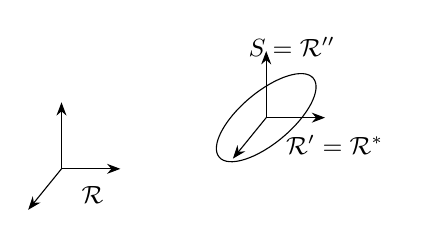
\begin{tikzpicture}[scale=.65]
\rep{\R}\begin{scope}[shift={(4,1)}]\draw[rotate=40] (0,0) ellipse(1.2 and .5);\rep{\R'=\R^*}\node[above] at (.5,1){$S=\R''$};\end{scope}
\end{tikzpicture}\end{center}
\[\Os=\vec\Omega_{S/\R^*}+\underbrace{\vec\Omega_{\R^*/\R}}_{=\vec0\text{ : translation}},\qquad
\Os=\vec\Omega_{S/\R^*}.\]
\end{exemple}
\begin{exemple}
\begin{minipage}{.38\linewidth}\centering
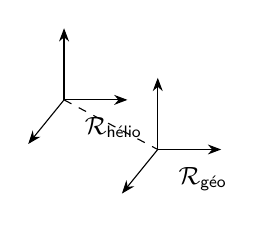
\begin{tikzpicture}[scale=.7]
\rep{\R_{\text{hélio}}}\draw[dashed] (0,0)--(1.7,-.9);
\begin{scope}[shift={(1.7,-.9)}]\rep{\R_{\text{géo}}}\end{scope}
\end{tikzpicture}
\end{minipage}\hfill\begin{minipage}{.59\linewidth}
$\R=\R_{\text{héliocentrique}}$,\\
$\R'=\R_{\text{géocentrique}}=\R^*_{\mathrm{Terre}}$,\\
$\R''=\R_{\mathrm{terrestre}}$.
\end{minipage}
\[\vec\Omega_{\mathrm{Terre}/\R_{\text{hélio}}}
=\vec\Omega_{\mathrm{Terre}/\R_{\text{géo}}}
+\underbrace{\vec\Omega_{\R_{\text{géo}}/\R_{\text{hélio}}}}_{=\vec0\text{ : translation}}.\]
\[\vec\Omega_{\mathrm{Terre}/\R_{\text{hélio}}}=\vec\Omega_{\mathrm{Terre}/\R_{\text{géo}}}.\]
On retrouve le jour sidéral : $23\ \mathrm h\ 56\ \mathrm{min}$.
\end{exemple}
\section{Composition des vitesses}
\subsection{Vitesse d'un point dans deux référentiels}
\begin{center}\deuxrep{1}\end{center}
On considère $\V{\R}(M)$ et $\V{\R'}(M)$. $O$ est un point fixe dans $\R$ et $O'$ un point fixe dans $\R'$.
\[\V{\R}(M)=\D{\overrightarrow{OM}}{\R},\qquad
\V{\R'}(M)=\D{\overrightarrow{O'M}}{\R'}.\]
Par changement d'origine,
\begin{align*}
\D{\overrightarrow{OM}}{\R}
&=\D{\overrightarrow{OO'}}{\R}+\D{\overrightarrow{O'M}}{\R}\\
&=\V{\R}(O')+\D{\overrightarrow{O'M}}{\R'}+\Om\wedge\overrightarrow{O'M}.
\end{align*}
\begin{cadre}
\[\V{\R}(M)=\V{\R'}(M)+\V{\R}(O')+\Om\wedge\overrightarrow{O'M}.\]
\end{cadre}
% Source : page 14.
\subsection{Loi de composition des vitesses}
Le point coïncident $P$ est le point fixe dans $\R'$ qui coïncide avec $M$ à un instant $t$.
Appliquons la formule à $P$ :
\[\V{\R}(P)=\underbrace{\V{\R'}(P)}_{=\vec0\text{ : }P\text{ fixe}}
+\V{\R}(O')+\Om\wedge\underbrace{\overrightarrow{O'P}}_{=\overrightarrow{O'M}\text{ : coïncidence}}.\]
\begin{cadre}[etoiles={\etoiles{5}}]
\[\V{\R}(P)=\V{\R}(O')+\Om\wedge\overrightarrow{O'M}=\vec v_e.\]
\end{cadre}
La vitesse d'entraînement est la vitesse du point coïncident.
La loi de composition des vitesses s'écrit :
\begin{cadre}[etoiles={\etoiles{5}}]
\[\V{\R}(M)=\V{\R'}(M)+\vec v_e(M).\]
\end{cadre}
\subsection{Cas d'un référentiel $\R'$ en translation par rapport à $\R$}
\begin{center}\deuxrep{0}\end{center}
$P$ coïncide avec $M$ à un instant $t$ et est fixe dans $\R'$. On cherche $\vec v_e(M)$ :
\[\vec v_e(M)=\V{\R}(P)=\V{\R}(O').\]
Tous les points fixes de $\R'$ ont la même vitesse dans $\R$.
\begin{cadre}[etoiles={\etoiles{5}}]\[\vec v_e(M)=\V{\R}(O').\]\end{cadre}
\subsection{Cas d'un référentiel $\R'$ en rotation uniforme autour d'un axe fixe dans $\R$}
\begin{center}\rotationfig\end{center}
\begin{cadre}[etoiles={\etoiles{5}}]
\[\vec v_e(M)=\V{\R}(P)=HM\,\Omega_{\R'/\R}\vec u_\theta=\Om\wedge\overrightarrow{HM}.\]
\end{cadre}
% Source : pages 16-17.
\section{Composition des accélérations}
\subsection{Accélération d'un point dans deux référentiels}
\begin{center}\deuxrep{1}\end{center}
\[\A{\R}(M)=\DD{\overrightarrow{OM}}{\R},\qquad
\A{\R'}(M)=\DD{\overrightarrow{O'M}}{\R'}.\]
On a déjà :
\[\V{\R}(M)=\V{\R'}(M)+\V{\R}(O')+\Om\wedge\overrightarrow{O'M}.\]
En dérivant dans $\R$,
\begin{align*}
\A{\R}(M)
&=\D{\V{\R'}(M)}{\R}+\underbrace{\D{\V{\R}(O')}{\R}}_{=\A{\R}(O')}\\
&\quad+\D{\Om}{\R}\wedge\overrightarrow{O'M}
+\Om\wedge\D{\overrightarrow{O'M}}{\R}\\
&=\underbrace{\D{\V{\R'}(M)}{\R'}}_{=\A{\R'}(M)}+\Om\wedge\V{\R'}(M)+\A{\R}(O')\\
&\quad+\D{\Om}{\R}\wedge\overrightarrow{O'M}
+\Om\wedge\left[\D{\overrightarrow{O'M}}{\R'}+\Om\wedge\overrightarrow{O'M}\right]\\
&=\A{\R'}(M)+\Om\wedge\V{\R'}(M)+\A{\R}(O')
+\D{\Om}{\R}\wedge\overrightarrow{O'M}\\
&\quad+\Om\wedge\V{\R'}(M)+\Om\wedge\left[\Om\wedge\overrightarrow{O'M}\right].
\end{align*}
\begin{cadre}[etoiles={\etoiles{2}}]
\[\begin{aligned}
\A{\R}(M)&=\A{\R'}(M)+2\Om\wedge\V{\R'}(M)\\
&\quad+\A{\R}(O')+\D{\Om}{\R}\wedge\overrightarrow{O'M}\\
&\quad+\Om\wedge\left(\Om\wedge\overrightarrow{O'M}\right).
\end{aligned}\]
\end{cadre}
% Source : page 18.
\subsection{Composition des accélérations}
Pour le point coïncident $P$,
\[\begin{aligned}
\A{\R}(P)&=\vec0+\vec0+\left(\A{\R}(O')+\D{\Om}{\R}\wedge\overrightarrow{O'M}\right.\\
&\qquad\left.+\Om\wedge\left(\Om\wedge
\underbrace{\overrightarrow{O'P}}_{=\overrightarrow{O'M}}\right)\right).
\end{aligned}\]
L'accélération d'entraînement est
\[\vec a_e(M)=\A{\R}(P).\]
\[\A{\R}(M)=\A{\R'}(M)+
\underbrace{2\Om\wedge\V{\R'}(M)}_{=\vec a_c(M)\text{ : accélération de Coriolis}}+\vec a_e(M).\]
\begin{cadre}[etoiles={\etoiles{5}}]
\[\A{\R}(M)=\A{\R'}(M)+\vec a_c(M)+\vec a_e(M).\]
\end{cadre}
Avec :
\begin{cadre}[etoiles={\etoiles{5}}]
\[\vec a_c(M)=2\Om\wedge\V{\R'}(M).\]
\end{cadre}
\begin{cadre}\[\vec a_e(M)=\A{\R}(P).\]\end{cadre}
% Source : pages 19-20.
\subsection{Cas d'un référentiel $\R'$ en translation par rapport à $\R$}
\begin{center}\deuxrep{2}\end{center}
\begin{cadre}[etoiles={\etoiles{4}}]
\[\vec a_e(M)=\A{\R}(P)=\A{\R}(O').\]
\end{cadre}
Tous les points de $\R'$ ont la même vitesse dans $\R$, donc la même accélération.
Comme $\Om=\vec0$, on a $\vec a_c=\vec0$.
\begin{cadre}[etoiles={\etoiles{4}}]\[\vec a_c(M)=\vec0.\]\end{cadre}
\subsection{Cas d'un référentiel $\R'$ en rotation uniforme autour d'un axe fixe dans $\R$}
\begin{center}\rotationfig\end{center}
\[\begin{aligned}
\vec a_e(M)&=\A{\R}(P)\\
&=-HM\,\Omega_{\R'/\R}^{2}\vec u_r+
HM\,\underbrace{\dot\Omega_{\R'/\R}}_{=0\text{ en rotation uniforme}}\vec u_\theta.
\end{aligned}\]
\begin{cadre}[etoiles={\etoiles{4}}]
\[\vec a_e(M)=-\Omega_{\R'/\R}^{2}\overrightarrow{HM}.\]
\end{cadre}
\[\vec a_c(M)=2\Om\wedge\V{\R'}(M).\]
% Source : pages 20-21.
\Needspace{55mm}\section*{Annexe}
\titr{Transformation de Galilée}
$\R'$ est en translation rectiligne uniforme. À $t=0$, $O=O'$ et $\overrightarrow{OO'}=vt\uy$.
\begin{center}\begin{tikzpicture}[scale=.75]
\foreach \q/\p in {0/,4/'}{\begin{scope}[shift={(\q,0)}]
\draw[->] (0,0)--(-.8,-1) node[below]{$x\p$};\draw[->] (0,0)--(1.4,0) node[right]{$y\p$};\draw[->] (0,0)--(0,1.5) node[above]{$z\p$};\node[below right] at (0,0){$O\p$};\node at (.8,-.6){$\R\p$};\end{scope}}
\node at (5.5,1.1){$\times M$};
\end{tikzpicture}\end{center}
\[\overrightarrow{OM}=\overrightarrow{OO'}+\overrightarrow{O'M},\qquad
\begin{cases}x=x',\\y=y'+vt,\\z=z'.\end{cases}\]
Le temps est absolu :
\[\vec u_x=\vec u_{x'},\qquad\vec u_y=\vec u_{y'},\qquad\vec u_z=\vec u_{z'}.\]
\[\begin{cases}\dot x=\dot x',\\\dot y=\dot y'+v,\\\dot z=\dot z'.\end{cases}\]
\[\V{\R}(M)=\V{\R'}(M)+v\uy.\]
On obtient le même résultat avec la loi de composition des vitesses.
\end{document}